\documentclass[11pt]{article}

%####### DON'T CHANGE MARGIN SETTINGS ###########
\newcommand{\keywordfont}{\textsc}
\newcommand{\keyword}[1]{%
  \marginpar{\raggedright\small\keywordfont{#1}}}
\reversemarginpar
\usepackage[a4paper, top=2.5cm, bottom=2.5cm, outer=2cm, inner=3.3cm, marginparwidth=72pt, heightrounded]{geometry}
%#################################

\usepackage{amsmath}
\usepackage{amssymb}
\usepackage{hyperref}
\usepackage{graphicx}
\usepackage{microtype}

\begin{document}

\Large
\begin{center}
\textbf{MA3K7 Week $3$ Rubric}
\\
Timothy Yap (2161367)
\end{center}
\normalsize



%-----------------------------------------------------------------------------------------------------------



\section{Entry}

 We begin with two numbers below $10$. \keyword{I know} This would include integers $0$ to $9$. The sequence starts with these two numbers and some 'rule' generates the next term. 

Finding this \keyword{I want} rule is the first thing we want. This is pivotal to figuring out the first part of the question as we need this rule to continue the bracelet and see what happens. Furthermore, it would allow us to begin finding out how many different bracelets there are.

 Before specialising, a notable sequence would be the Fibonacci sequence. It begins with $0$ and $1$ and the next number is just the addition of the previous two terms. Giving $0, 1, 1, 2, 3, 5, 8, 13...$ as the first $8$ terms. The Fibonacci sequence also connect to the Golden ratio and the Pascal's triangle so our sequence may also show connections to other mathematical properties.


The example \keyword{Specialise} given is 
\[
1 \rightarrow 5 \rightarrow 6 \rightarrow 1 \rightarrow 7 \rightarrow 8 \rightarrow 5 \rightarrow 
\]
with $1$ and $5$ being the starting two numbers.

We observe that $6 = 5 + 1$ but then $1 \neq 6 + 5$. \keyword{Stuck} So the same rule from the Fibonacci sequence doesn't apply and requires some modification.

A possible fix would be to \keyword{AHA} alternate between addition and subtraction. Now we get $1 = 6 - 5$ for every other term. 
This does \keyword{Check} continue with $7 = 1 + 6$ but then we get $8 \neq 7 - 1$ so we're back to square one. \keyword{Stuck}

Writing all the terms in a table may help give some insights, \keyword{Specialise}
but before we can do that, \keyword{Introduce} we will denote a term by $x_n$ depending on its position (starting at 0) in the sequence. For example, 1 is $x_0$ and 5 is $x_1$.

\begin{table} [h]
    \centering
    \begin{tabular}{c|c|c|c}
         $x_n$ & $x_{n-1}$ & $x_{n-2}$ & $x_{n-1}$ + $x_{n-2}$ \\
         6 & 5 & 1 & 6 \\
         1 & 6 & 5 & 11 \\
         7 & 1 & 6 & 7 \\
         8 & 7 & 1 & 8 \\
         5 & 8 & 7 & 15 \\
    \end{tabular}
\end{table}

First we notice that \keyword{AHA} 11 and 15 are above 10 and when taking modulo 10 they are equivalent to 1 and 5 respectively. This could relate to the two starting numbers also being below 10. We now have a new rule of addition under modulo 10, being similar to Fibonacci just with modulo 10 and a multitude of starting pairs.



%-----------------------------------------------------------------------------------------------------------



\section{Attack}
Following from the Entry, we use the rule we discovered \keyword{Try} to continue the sequence and observe any patterns.

\[
1 \rightarrow 5 \rightarrow 6 \rightarrow 1 \rightarrow 7 \rightarrow 8 \rightarrow 5 \rightarrow 3 \rightarrow 8 \rightarrow 1 \rightarrow 9 \rightarrow 0 \rightarrow 9 \rightarrow 9 \rightarrow 8 \rightarrow 7 \rightarrow 5 \rightarrow 2 \rightarrow 7 \rightarrow  ...
\]
It seems that this bracelet is \keyword{Stuck} tedious to calculate by hand. Some Python code may be helpful in computing such a sequence. \keyword{AHA} Using the code we get the sequence as below and a sequence of 60 terms. 

\begin{align*}
1 \ 5 \ 6 \ 1 \ 7 \ 8 \ 5 \ 3 \ 8 \ 1 \ 9 \ 0 \ 9 \ 9 \ 8 \ 7 \ 5 \ 2 \ 7 \ 9 \\
6 \ 5 \ 1 \ 6 \ 7 \ 3 \ 0 \ 3 \ 3 \ 6 \ 9 \ 5 \ 4 \ 9 \ 3 \ 2 \ 5 \ 7 \ 2 \ 9 \\
1 \ 0 \ 1 \ 1 \ 2 \ 3 \ 5 \ 8 \ 3 \ 1 \ 4 \ 5 \ 9 \ 4 \ 3 \ 7 \ 0 \ 7 \ 7 \ 4   
\end{align*}


Something to note about this sequence is that it loops after 7 and 4 as the next two consecutive terms are 1 and 5. Thus repeating from the beginning and also giving meaning to the term bracelet. Picking any pair in the sequence will generate the same sequence until 1 and 5 are consecutive terms. \keyword{Check} We can check by picking 1 and 1 from the last row.

\[
1 \rightarrow 1 \rightarrow 2 \rightarrow 3 \rightarrow 5 \rightarrow 8 \rightarrow 3 \rightarrow 1 \rightarrow 4 \rightarrow 5 \rightarrow 9 \rightarrow 4 \rightarrow 3 \rightarrow 7 \rightarrow 0 \rightarrow 7 \rightarrow 7 \rightarrow 4 \rightarrow 1 \rightarrow 5
\]

This gives inspiration to the first conjecture:

Any two consecutive numbers on a bracelet will produce the same bracelet. \keyword{Conjecture}

As we know the rule holds for any two pairs, \keyword{Justification} picking any pair on this bracelet will produce the same bracelet up to ordering of starting position. Using the above check, once 1 and 5 are reached, the same bracelet will be produced and repeated. This can be checked with Python code \keyword{Check} where each pair can be printed and checked if it has 1 and 5 in its sequence. We can observe that the sequence is repeated with the number of terms staying the same, at 60. 

This motivates us to \keyword{Introduce} introduce \textit{length} as the number of terms in a sequence. In the case that the sequence doesn't end, we'll say it has an infinite length. Length may or may not be unique to each bracelet but at least we can check bracelets between each other when discussing the next question: "How many different bracelets are there?".

Again using Python, we can iterate over all pairs $(a, b)$ such that $a, b \in \{0, 1, 2, ... 8, 9\}$. This gives us 6 different bracelets (again up to ordering of starting pair). All bracelets are listed as below with their name being the first index that produced that bracelet:

\begin{description}
    \item[Bracelet (0, 0)] with length 1
    \item 0 \ 0
    \item[Bracelet (0, 1)] with length 60
    \item 0 \ 1 \ 1 \ 2 \ 3 \ 5 \ 8 \ 3 \ 1 \ 4 \ 5 \ 9 \ 4 \ 3 \ 7 \ 0 \ 7 \ 7 \ 4 \ 1 \ 5 \ 6 \ 1 \ 7 \ 8 \ 5 \ 3 \ 8 \ 1 \ 9 \ 0 \ 9 \ 9 \ 8 \ 7 \ 5 \ 2 \ 7 \ 9 \ 6 \ 5 \ 1 \ 6 \ 7 \ 3 \ 0 \ 3 \ 3 \ 6 \ 9 \ 5 \ 4 \ 9 \ 3 \ 2 \ 5 \ 7 \ 2 \ 9 \ 1 \ 0 \ 1 \ 
    \item[Bracelet (0, 2)] with length 20
    \item 0 \ 2 \ 2 \ 4 \ 6 \ 0 \ 6 \ 6 \ 2 \ 8 \ 0 \ 8 \ 8 \ 6 \ 4 \ 0 \ 4 \ 4 \ 8 \ 2
    \item[Bracelet (0, 5)] with length 3
    \item 0 \ 5 \ 5 
    \item[Bracelet (1, 3)] with length 12
    \item 1 \ 3 \ 4 \ 7 \ 1 \ 8 \ 9 \ 7 \ 6 \ 3 \ 9 \ 2
    \item[Bracelet (2, 6)] with length 4
    \item 2 \ 6 \ 8 \ 4 
\end{description}

First thing to note is that the $(0, 0)$ bracelet could have an ambiguous length. With our previous definition, the 'number of terms in a sequence', it could be said that this bracelet has either a length of 2 or 3 as the rule of addition module 10 must be done once. Another observation is that $60 + 20+ 3 + 12 + 4 = 99$, so we may want to change our definition to be more accurate and have the $(0, 0)$ bracelet with length 1. An improved idea of \keyword{Introduce} length would be the 'number of times the rule is applied until returning to the original pair'. Thus leaving the other bracelets with the same length and now giving the sum of all the lengths to be $1 + 60 + 20+ 3 + 12 + 4 = 100$.
    

By finding all the bracelets, we eliminate the possibility for the situation below where a possible pair of numbers generate a bracelet without generating itself as shown below. This may be possible but not for our given restrictions and will be explored more in the Review stage.

\begin{figure}[h] % h means put the figure "here"
   \centering
   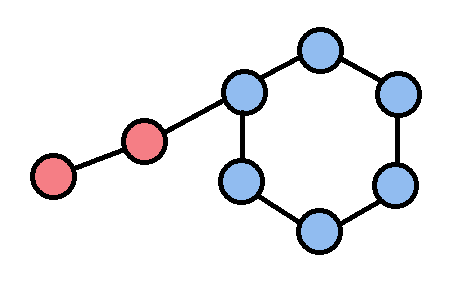
\includegraphics[width=2in]{samplefig2.png} 
   \caption{Two terms generating seperate Bracelet}
   \label{myfig}
\end{figure}



%-----------------------------------------------------------------------------------------------------------



\section{Review}

I have found \keyword{Check}  that the bracelets loop back creating a repeating sequence and that there are exactly 6 different bracelets given our restriction onto the positive integers below 10. 

By testing possible rules \keyword{Reflect} I was able to find one that worked with the initial sequence. This was a key step as discovering the pattern allowed me to begin exploring the other parts of the question. Even if the rule I initially tested was incorrect, it allowed me to refocus my efforts and possibly could be used in extensions.

At the beginning, my knowledge of length was limited so I was only able to give a definition of length based on what I knew at the time. After attacking the question, the definition of length changed to better fit special cases, specifically the (0, 0) case. 

During this assignment, I introduced the notation $x_n$ which became less useful once the sequence repeated and was generated by different pairs of the same sequence. As depending on the starting pair, 1 and 5 will be $x_n$ and $x_{n+1}$. However, the notation is still useful when dealing with extensions of this problem where the sequence doesn't repeat, for example using transcendental numbers as the starting pair.

Lastly, Python has been used to help calculate sequences, the length of the sequences, check for the uniqueness for each sequence. Without it calculations by hand would take a tedious amount of time. Python can also easily be change to fit in extensions and generalisations. Which leads to the next part.

There are multiple ways of extend this idea of bracelets and sequences with two numbers. \keyword{Extend} First we may try different values of $x$ so our rule changes to addition modulo $x$. Possibly extending the starting numbers to be greater or lesser than 10. This could change the number of bracelets. For example, staying in modulo 10 if the starting value had to be 3 and below, we would not be able to generate $0 \ 5 \ 5$ and $ 2 \ 6 \ 8 \ 4$. Thus giving 4 bracelets instead. Below is a list of possible extensions to the question:

\begin{itemize}
    \item Changing addition modulo 10 to addition modulo $x$
    \item Starting numbers must be in the interval $[a, b]$
    \item Addition of previous $y$ terms
    \item Using starting terms in $\mathbb{Q}, \mathbb{R}, \mathbb{C}, \mathbb{F}_n$ or even above the value for $x$
    \item Similar to my initial guess for the rule, potentially changing from addition to subtraction for odd and even terms.
    \item Going further we may change the operation all together
\end{itemize}

By choosing starting numbers above the $x$ value for our modular addition, we can create a bracelet similar to Figure 1. For example below;

\[
17 \rightarrow 14 \rightarrow 1 \rightarrow 5 \rightarrow 6 \rightarrow 1 \rightarrow 7 \rightarrow 8 \rightarrow 5 \rightarrow 3 \rightarrow 8 \rightarrow 1 \rightarrow 9 \rightarrow 0 \rightarrow 9 \rightarrow 9 \rightarrow 8 \rightarrow 7 \rightarrow 5  ...
\]

Thus it is possible, as long as we remove certain restrictions from our problem.

Using some of the above suggestions for extensions, I coded a Python function that takes two starting numbers and an $x$ value for the addition modulo $x$. With my code, I found the following information:

\begin{table} [h]
    \centering
    \begin{tabular}{cccc}
        mod $x$ & Number of Bracelets & Length of Bracelets & Sum of Lengths\\
        1 & 1 & 1 & 1\\  
        2 & 2 & 1, 3 & 4\\
        3 & 2 & 1, 8 & 9\\
        4 & 4 & 1, 6, 3, 6 & 16\\
        5 & 3 & 1, 20, 4 & 25\\
        6 & 4 & 1, 24, 8, 3 & 36\\
        7 & 4 & 1, 16, 16, 16 & 49\\
        8 & 8 & 1, 12, 6, 12, 3, 6, 12, 12, 8 & 64\\
        9 & 5 & 1, 24, 8, 24, 24 & 81\\
        10 & 6 & 1, 60, 20, 3, 12, 4, 6 & 100\\      
    \end{tabular}
\end{table}

This just changed the value for modular addition and starting values but highlights how even one change creates very different bracelets. From this table we can see our new definition of length lets the sum of lengths be equal to the number of starting position. We can also observe that not all lengths are unique, in fact they repeat for certain values.

Exploring different changes may result in very unique bracelets, some may produce very unique alternating patterns, some may never repeat, and potentially relate to other mathematical properties, the same way the Fibonacci sequence relates to the Golden ratio.


\section*{Supplementary material}
The code for this assignment can be found on my GitHub page:  \url{https://github.com/LazyTim/MA3K7/blob/main/MA3K7%20-%20Assignment1.ipynb}.

\end{document}
